%-----------------------------------------------------------------------------------------------------------------------------------------------%
%	The MIT License (MIT)
%
%	Copyright (c) 2021 Jitin Nair
%
%	Permission is hereby granted, free of charge, to any person obtaining a copy
%	of this software and associated documentation files (the "Software"), to deal
%	in the Software without restriction, including without limitation the rights
%	to use, copy, modify, merge, publish, distribute, sublicense, and/or sell
%	copies of the Software, and to permit persons to whom the Software is
%	furnished to do so, subject to the following conditions:
%	
%	THE SOFTWARE IS PROVIDED "AS IS", WITHOUT WARRANTY OF ANY KIND, EXPRESS OR
%	IMPLIED, INCLUDING BUT NOT LIMITED TO THE WARRANTIES OF MERCHANTABILITY,
%	FITNESS FOR A PARTICULAR PURPOSE AND NONINFRINGEMENT. IN NO EVENT SHALL THE
%	AUTHORS OR COPYRIGHT HOLDERS BE LIABLE FOR ANY CLAIM, DAMAGES OR OTHER
%	LIABILITY, WHETHER IN AN ACTION OF CONTRACT, TORT OR OTHERWISE, ARISING FROM,
%	OUT OF OR IN CONNECTION WITH THE SOFTWARE OR THE USE OR OTHER DEALINGS IN
%	THE SOFTWARE.
%	
%
%-----------------------------------------------------------------------------------------------------------------------------------------------%

%----------------------------------------------------------------------------------------
%	DOCUMENT DEFINITION
%----------------------------------------------------------------------------------------

% article class because we want to fully customize the page and not use a cv template
\documentclass[a4paper,12pt]{article}

%----------------------------------------------------------------------------------------
%	FONT
%----------------------------------------------------------------------------------------

% % fontspec allows you to use TTF/OTF fonts directly
% \usepackage{fontspec}
% \defaultfontfeatures{Ligatures=TeX}

% % modified for ShareLaTeX use
% \setmainfont[
% SmallCapsFont = Fontin-SmallCaps.otf,
% BoldFont = Fontin-Bold.otf,
% ItalicFont = Fontin-Italic.otf
% ]
% {Fontin.otf}

%----------------------------------------------------------------------------------------
%	PACKAGES
%----------------------------------------------------------------------------------------
\usepackage{url}
\usepackage{parskip} 	

%other packages for formatting
\RequirePackage{color}
\RequirePackage{graphicx}
\usepackage[usenames,dvipsnames]{xcolor}
\usepackage[scale=0.9]{geometry}

%tabularx environment
\usepackage{tabularx}

%for lists within experience section
\usepackage{enumitem}

% centered version of 'X' col. type
\newcolumntype{C}{>{\centering\arraybackslash}X} 

%to prevent spillover of tabular into next pages
\usepackage{supertabular}
\usepackage{tabularx}
\newlength{\fullcollw}
\setlength{\fullcollw}{0.47\textwidth}

%custom \section
\usepackage{titlesec}				
\usepackage{multicol}
\usepackage{multirow}

%CV Sections inspired by: 
%http://stefano.italians.nl/archives/26
\titleformat{\section}{\Large\scshape\raggedright}{}{0em}{}[\titlerule]
\titlespacing{\section}{0pt}{10pt}{10pt}

%for publications
\usepackage[style=authoryear,sorting=ynt, maxbibnames=2]{biblatex}

%Setup hyperref package, and colours for links
\usepackage[unicode, draft=false]{hyperref}
\definecolor{linkcolour}{rgb}{0,0.2,0.6}
\hypersetup{colorlinks,breaklinks,urlcolor=linkcolour,linkcolor=linkcolour}
\addbibresource{citations.bib}
\setlength\bibitemsep{1em}

%for social icons
\usepackage{fontawesome5}

%debug page outer frames
%\usepackage{showframe}

%----------------------------------------------------------------------------------------
%	BEGIN DOCUMENT
%----------------------------------------------------------------------------------------
\begin{document}

% non-numbered pages
\pagestyle{empty} 

%----------------------------------------------------------------------------------------
%	HEADING
%----------------------------------------------------------------------------------------

\begin{minipage}[c]{2.5cm}
    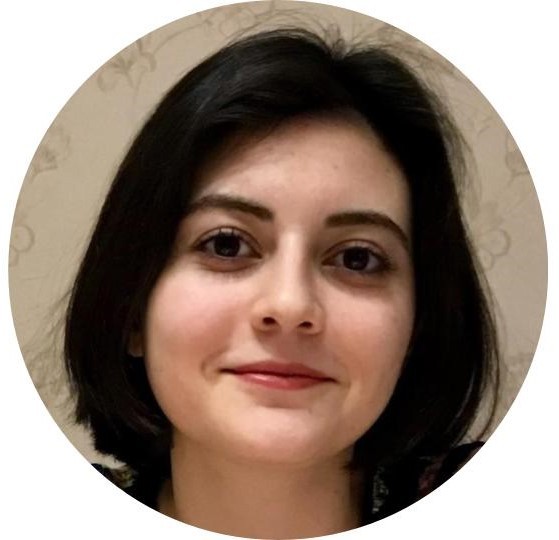
\includegraphics[width=2.5cm]{./avatar/avatar4.jpg}
\end{minipage}%
\hspace{1em}
\begin{minipage}[c]{\dimexpr\linewidth-2.5cm-15em\relax}
    \Huge{Arghavan Aslani}
\end{minipage}%
\begin{minipage}[c]{0.3\linewidth}
    \href{https://github.com/arghavanaslani}{\raisebox{-0.05\height}\faGithub\ github.com/arghavanaslani} \\ 
    \href{https://www.linkedin.com/in/arghavan-aslani/}{\raisebox{-0.05\height}\faLinkedin\ arghavan-aslani} \\ 
    \href{mailto:aslaniarghavan@gmail.com}{\raisebox{-0.05\height}\faEnvelope \ asaniarghavan@gmail.com} \\ 
    \href{tel:+989388687792}{\raisebox{-0.05\height}\faMobile \ +98.938.868.7792}
\end{minipage}

%----------------------------------------------------------------------------------------
%	EDUCATION
%----------------------------------------------------------------------------------------
\section{Education}
\begin{tabularx}{\linewidth}{@{}X r@{}}
    \textbf{B.Sc. in Electrical Engineering, University of Tehran, Tehran, Iran} & \textbf{Sep. 2017 - Sep. 2022} \\
    \multicolumn{2}{@{}X@{}}{\emph{Specialization in Control Systems}} \\
\end{tabularx}

\begin{tabularx}{\linewidth}{@{}X r@{}}
    {Overall GPA: 15.24/20} & \hfill \href{}{} \\[3.75pt]
    {Member of BTCS (Brain Tech and Cognitive Science Club)} & \hfill \href{}{} \\[3.75pt]
    {Performer and Member of Council at Performing Arts Club} & \hfill \href{https://www.instagram.com/fanni_theater/}{Link to Instagram Page} \\[3.75pt]
\end{tabularx}

%----------------------------------------------------------------------------------------
% EXPERIENCE SECTIONS
%----------------------------------------------------------------------------------------

%Experience
\section{Experience}

\begin{tabularx}{\linewidth}{@{}X r@{}}
    \textbf{Crowd Cognition group, LMU — Research Assistant} & \hfill Apr. 2022 - present \\[3.75pt]
    \href{https://crowdcognition.net/}{\raisebox{-0.05\height}\faGlobe\ crowdcognition.net} \\
\end{tabularx}
\begin{tabularx}{\linewidth}{@{}X r@{}}
    {Conducted multiple data collections using the Pupil Invisible eye-tracker from Pupil Labs and created a customized guide for data collection assistants.} & \hfill \href{https://crowd-cognition.github.io/Pupil-Invisible-Eye-Tracking-Data-Guide/}{Link to Guide} \\[3.75pt]
    {Utilized data analytics techniques (statistical tests, similarity metrics, ... .)} & \hfill \href{https://github.com/arghavanaslani/islamic_art_pilot_CG}{Link to Code} \\[3.75pt]
    {Created data visualization based on the analysed data.} & \hfill \href{https://github.com/arghavanaslani/MOT_questionnaire}{Link to Code} \\[3.75pt]
    {Developed application to track and illustrate gaze data in real-time.} & \hfill \href{https://github.com/arghavanaslani/livegaze}{Link to Code} \\[3.75pt]
\end{tabularx}

\vspace{\baselineskip} 

\begin{tabularx}{\linewidth}{@{}X r@{}}
    \textbf{ESLAB, University of Tehran — Lead Reseach Assistant} & \hfill July 2021 - August 2022 \\[3.75pt]
    \href{https://www.linkedin.com/company/eng-sci-lab/}{\raisebox{-0.05\height}\faLinkedin\ www.linkedin.com/company/eng-sci-lab} \\
\end{tabularx}

\begin{tabularx}{\linewidth}{@{}X r@{}}
    {Developed a robot 2-DOF robot "Spider-Paint" that is able to get a picture as input and draw/print it on a white-board using a marker.} & \hfill \href{https://github.com/arghavanaslani/spider-paint/blob/'spider-paint'/README.md}{Link to Videos} \\[3.75pt]
    {Designed an algorithm in C to control two stepper motors on vertical plan using a single Arduino.} & \hfill \href{https://github.com/arghavanaslani/spider-paint}{Link to Code} \\[3.75pt]
    {Authored a paper that has been accepted by the ISME Conference 2022.} & \hfill \href{https://civilica.com/doc/1468825/}{Link to Paper} \\[3.75pt]
\end{tabularx}

\vspace{\baselineskip} 

\begin{tabularx}{\linewidth}{@{}X r@{}}
    \textbf{CLIC, University of Tehran — Market Analyst} & \hfill July 2019 - Sep 2019 \\[3.75pt]
\end{tabularx}

\begin{tabularx}{\linewidth}{@{}X r@{}}
    {Conducted in-depth analysis to identify optimal markets for eye-tracking devices.} & \hfill \href{}{} \\[3.75pt]
    {Scheduled and facilitated meetings with potential customes.} & \hfill \href{}{} \\[3.75pt]
    {Prepared and delivered weekly progress reports on the analysis.} & \hfill \href{}{} \\[3.75pt]
\end{tabularx}

%----------------------------------------------------------------------------------------
% EPROJECTS
%----------------------------------------------------------------------------------------

%Projects
\section{Projects}

\begin{tabularx}{\linewidth}{ @{}l r@{} }
\textbf{Web Scraping for Job Advertisements in https://jobvision.ir} & \hfill \href{https://github.com/arghavanaslani/JobAdDB}{Link to Code} \\[3.75pt]
\multicolumn{2}{@{}X@{}}{Developed in Python.
Utilized BeautifulSoup, pandas, and requests for web scraping and data processing.
Created a custom database due to the unavailability of existing datasets in the field.}  \\
\end{tabularx}

%----------------------------------------------------------------------------------------
%	CERTIFICATIONS
%----------------------------------------------------------------------------------------

\section{Certifications}

\begin{tabularx}{\linewidth}{ @{}l r@{} }
{Task-Orienred Course in Data Analysis with Python} & \hfill \href{https://quera.org/certificate/7p1aeaOn/}{Link to Certificate} \\[3.75pt]
\multicolumn{2}{@{}X@{}}{}  \\
\end{tabularx}

\begin{tabularx}{\linewidth}{ @{}l r@{} }
{Computational Neuroscience, Neuromatch Academy} & \hfill \href{https://portal.neuromatchacademy.org/certificate/ee23deef-9e73-4233-8c46-6e85375d9f1b}{Link to Certificate} \\[3.75pt]
\multicolumn{2}{@{}X@{}}{}  \\
\end{tabularx}

%----------------------------------------------------------------------------------------
%	PUBLICATIONS
%----------------------------------------------------------------------------------------

\section{Publications}

\begin{tabularx}{\linewidth}{ @{}l r@{} }
{Design, Fabrication and Control of 2 DoF Robot in Vertical Plan} & \hfill \href{https://civilica.com/doc/1468825/}{Link to Paper} \\[3.75pt]
\multicolumn{2}{@{}X@{}}{}  \\
\end{tabularx}

%----------------------------------------------------------------------------------------
%	SKILLS
%----------------------------------------------------------------------------------------
\section{Technical Skills}
\begin{tabularx}{\linewidth}{@{}l X@{}}
    Programming Languages &  \normalsize{Python, C, C++, SQL, MATLAB, HTML, CSS, JavaScript, R}\\
    miscellaneous &  \normalsize{Linux, Git, Windows, LATEX, Microsoft Office}\\  
\end{tabularx}


\end{document}
